\paragraph{}
  D’après LE PETIT LAROUSSE ILLUSTRE 2010, l’intrusion est définie comme <<l’action de s’introduire sans y être invité dans un lieu, une société, un groupe, un système informatique. C’est aussi l’action d’intervenir dans un domaine où l’on n'a aucun titre à le faire>>. Cette définition de l’intrusion s’applique aussi en informatique \footnote{ Le petit Larousse Illustré 2010.} \cite{b}. En effet, l’intrusion en informatique est définie comme étant toute utilisation d’un système informatique à des fins autres que celles prévues, généralement après acquisition de privilèges de façon illégitime.
\paragraph{}
  L'arrivée d'Internet a apporté une grande révolution dans le monde mais aussi a entraîné une kyrielle de problèmes dans le domaine de la protection de la vie privée.  Ainsi des personnes appelées hackers arrivent à prendre possesion de tout un système d'information et à le paralyser.

  
\subsection{Notion de hacker et de cracker}
  \paragraph{}
    Un hacker est une personne qui, par jeu, goût du défi ou souci de notoriété, cherche à contourner les protections d'un logiciel, à s'introduire frauduleusement dans un système ou un réseau informatique. \cite{A} \footnote{Recommandation officielle : fouineur.}.\\Un cracker, quant à lui, s’introduit tout aussi frauduleusement dans un système informatique pour en entraver ou en fausser le fonctionnement. Son action est souvent plus dévastatrice.
	

\subsection{Mode opératoire d'une intrusion informatique}
  \paragraph{}
    Un test d’intrusion peut être décomposé en une suite d’étapes ou phases. Lorsqu’elles sont réunies, ces étapes forment une méthodologie complète pour mener à bien un test d’intrusion. L’établissement d’une méthodologie permet de décomposer une procédure complexe en une suite de tâches gérables de taille plus réduite. Ainsi nous regroupons cette méthodologie en quatre étapes qui sont \textbf{la reconnaissance}, \textbf{les scans}, \textbf{l'exploitation}, \textbf{la postexploitation et le maintien d'accès} \footnote{La post exploitation et le maintien d'accès forment une étape.}\cite{c}.
      
  \subsubsection{La reconnaissance}
    \paragraph{}
      La reconnaissance, ou recueil d’informations, est probablement la plus importante des quatre phases. Plus le hacker passe du temps à collecter des informations sur sa cible, plus les phases suivantes auront une chance de réussir\cite{c}. En effet la reconnaissance permet de connaitre la cible dans les détails, de connaître les points forts et surtout les points faibles afin de notifier les prochaines possibilités d'attaque.

  \subsubsection{Les scans}
    \paragraph{}
      Les scans sont des procédés ayant pour objectif d’identifier les systèmes actifs et les services qui existent sur les systèmes scannés. Dans ce cadre, le hacker prend le soin de vérifier l'activité d'un système, de trouver les portes ouvertes (les ports), de vérifier les processus tournant sur le système et d'aller à la recherche des vulnérabilités. Ce stade requiert une compréhension plus avancée des systèmes informatiques pour mieux comprendre les résultats recueillis \footnote{Informations recueillis au cours du scan}\cite{c}.
      
  \subsubsection{L'exploitation}
    \paragraph{}
      En termes simples, l’exploitation consiste à obtenir un contrôle sur un système. Toutefois, il est à notifier que tout exploit ne conduit pas à la compromission intégrale d’un système. Un hacker peut se servir donc d'un exploit pour télécharger des contenus dont il ne détient pas la propriété pendant qu'un autre utilise un exploit pour crypter les fichiers du système. L'utilisation de l'un des exploits \footnote{Un exploit est le moyen par lequel un attaquant, ou un pentester en l’occurrence, profite d’un défaut dans un système, une application ou un service.} dépend donc de l'objectif visé par le hacker \cite{E}.

  \subsubsection{Post exploitation et maintien d’accès}
    \paragraph{}
      Cette étape consiste à couvrir les traces de l'intrus agissant afin de ne pas se faire repérer \cite{E}. Il permet aussi à ce dernier de facilliter ses prochains accès à la machine victime de ses attaques par l'installation de portes dérobées communément appelées "Backdoor". Ainsi, il n'aura plus besoin de reprendre toutes les étapes de son processus pour accéder à la machine dont il prend le contrôle.\\ \\
      

\begin{figure}[H]
  \begin{center}
    %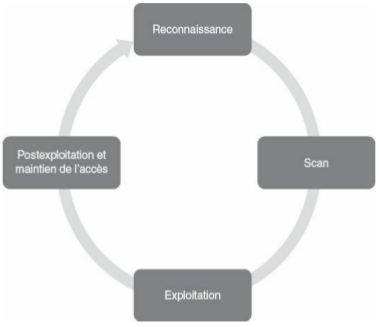
\includegraphics[scale=0.5]{images/zeh_cycle.png}
  \end{center}
  \caption[Représentation cyclique de la méthodologie ZEH.]
    {Méthodlogie ZEH, Patrcick Engebretson, "Les bases du hacking", PEARSON 2013}
    \label{Methodologie d'intrusion}
\end{figure}

\paragraph{}
  La méthodologie d'attaque étant cernée, nous allons maintenant présenter les différentes sortes d'attaque auxquelles sont confontrés les systèmes informatiques.	    
		    
\subsection{Quelques exemples d'attaques informatiques}
  \paragraph{}
    Parmi les attaques les plus connues, on peut citer les techniques de déni de service (DoS), l'usurpation d'adresse IP, l'usurpation du DNS \textit{Domain Name Server}, l'ingénierie sociale.		    
	
  \subsubsection{Le deni de service}
    \paragraph{}
      D'une manière générale, on parle de déni de service quand une personne ou une organisation est privée d'un service utilisant des ressources qu'elle est en droit d'avoir en temps normal \cite{B}. On trouvera par exemple des dénis de service touchant le service de courrier électronique, d'accès à Internet, de ressources partagées (pages Web), ou tout autre service à caractère commercial comme Yahoo ou EBay.\\ \\
      Quoiqu'il en soit, le déni de service est un type d'attaque qui coûte généralement très cher puisqu'il interrompt le cours normal des transactions pour une entreprise; les sommes et les enjeux sont énormes et cela ne peut aller qu'en s'aggravant tant que des parades réellement efficaces n'auront pas été trouvées.\\ \\
      Il existe plusieurs moyens pour parvenir à un déni de service. Nous ne parlerons que de trois types dont l'attaque avec les paquets \textbf{XMAS}, l'attaque \textbf{Smurf}, et l'attaque par \textbf{Syn flooding}.

      \subparagraph*{L'attaque avec paquets XMAS.}
	Un paquet XMAS ou Christmas Tree est un paquet dans lequel les drapeaux \textit{(flag)} de tout protocole sont définis. Les bits FIN, URG et PSH dans l'en-tête TCP de ce type de paquet sont définis. Ce paquet s'appelle paquet Christmas Tree, car tous les champs d'en-tête sont éclairés c'est à dire activés comme un arbre de noël. Ce type de paquet nécessite beaucoup plus de traitements que les paquets habituels, de sorte que le serveur alloue un grand nombre de ressources pour ce paquet. Par conséquent, cela peut être utilisé pour effectuer une attaque DoS sur le serveur.

      \subparagraph{L'attaque Smurf.}
	L'attaquant ici envoie un grand nombre de paquets de diffusion d'écho ICMP, avec des adresses IP source falsifiées par rapport à l'adresse IP de la cible. Toutes les machines du réseau reçoivent ce message de diffusion et répondent à la cible avec un paquet de réponse d'écho.

      \subparagraph{Le syn flooding.}
	Lors de l'initialisation d'une connexion TCP entre un client et un serveur, un échange de messages a lieu. Le principe est celui du three-way handshake, qui dans le cas d'une connexion normale sans volonté de nuire, se déroule en trois étapes :
	\begin{enumerate}
	  \item le client demande une connexion en envoyant un message SYN (pour synchronize) au serveur;
	  \item le serveur accepte en envoyant un message SYN-ACK (synchronize-acknowledgment) vers le client;
	  \item le client répond à son tour avec un message ACK (acknowledgment) ; la connexion est alors établie.
	\end{enumerate}
	
	\begin{figure}[H]
	  \begin{center}
	    %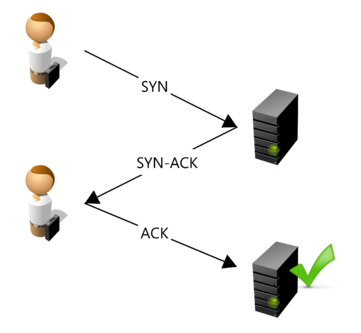
\includegraphics[scale=0.5]{images/handshake.png}
	  \end{center}
	  \caption[TCP handshake]{3 ways Handshake}
	  \label{Mécanisme d'établissement de connexion TCP}
	\end{figure}
	
	L'attaquant peut créer un grand nombre de requêtes SYN forgées qui ont leurs adresses IP source falsifiées et l'envoyer à la cible. La cible répond avec SYN-ACK et alloue ses ressources pour la connexion, mais ne reçoit jamais la réponse ACK. Les ressources de la machine cible sont épuisées et elles ne permettent pas de répondre à d'autres demandes de  machines légitimes.

	\subsubsection{L'usurpation d'adresse IP}
	  \paragraph{}
	    L'« usurpation d'adresse IP » (également appelée mystification ou en anglais \textit{IP Spoofing}) est une technique consistant à remplacer l'adresse IP de l'expéditeur d'un paquet IP par l'adresse IP d'une autre machine.
	    Cette technique permet ainsi à un pirate d'envoyer des paquets de façon anonyme. Il ne s'agit pas pour autant d'un changement d'adresse IP, mais d'une mascarade de l'adresse IP au niveau des paquets émis \cite{F}.

	\subsubsection{L'usurpation DNS}
	  \paragraph{}
	    Il s'agit de corrompre le cache du serveur DNS \textit{ Domain Name Server} afin de faire croire à une machine qu'un nom de machine est relatif à une fausse adresse donnée. Ainsi donc les communications vers la machine ciblée sont redirigées vers celle dont l'adresse est portée en avant.

	\subsubsection{Ingénierie sociale}
	  \paragraph{}
	  L'ingénierie sociale est une attaque qui s'appuie essentiellement sur les relations humaines pour inciter de façon détournée à enfreindre les procédures de sécurité \cite{social}. L’ingénierie sociale fait partie des techniques les plus simples, mais aussi les plus efficaces pour entrer dans un système sécurisé à grande échelle. En effet le système aura beau être sécurisé avec les moyens les plus sophistiqués, une seule information divulguée d'un utilisateur aura suffi pour mettre le système à terre. Il s'agit d'une arme très forte résultant de l'étude de l'être humain, de ses passions, de ses désirs. Cette forme d'attaque est très dévastatrice en fonction de l'importance des informations tirées.\\
	  Face à ces différentes menaces, différentes solutions sont nées. Nous allons en présenter quelques-unes.
		        	    
    \subsection{Les applications basées sur la détection et la prévention d'intrusion}
      \paragraph{}
	Plusieurs systèmes ont vu le jour en raison des attaques qui sévissent de jour en jour. Il s'agit des IDS (\textit{Intrusion Detection System}), des IPS (\textit{Intrusion Prevention System}), des firewall (Pare-feu), des antivirus pour ne citer que ceux là.
	
      \subsubsection{Les systèmes de détection d'intrusion}
	\paragraph{}
	  Un système de détection d’intrusion \textit{Intrusion Detection System (IDS) en anglais} est comparable à une alarme domestique contre les voleurs. Si une tentative de pénétration non avenue est découverte, une alerte sera déclenchée.
	  La fiabilité d'un tel système dépend de la puissance des capteurs à détécter les événements pour lequels ils ont été mis en place avec une marge d'erreur minimisée. 
	  Certains termes sont souvent employés quand on parle d’IDS et il sied de les  comprendre. Il s'agit notamment du faux positif et du faux négatif.\\
	  Un faux positif est une alerte provenant d’un IDS mais qui ne correspond pas à une attaque réelle, tandis qu'un faux négatif est une intrusion réelle qui n’a pas été détectée par l’IDS.

    Un systéme de détection d'intrusion se base sur trois éléments particuliers:
    \begin{itemize}
      \item la sonde qui collecte les informations sur le système;
      \item l'analyseur qui traite ces informations afin de détecter les possibilités d'attaque;
      \item la réponse qui est la solution apportée à la menace détectée.
    \end{itemize}    

    \textbf{Quelques exemples d'IDS}
    
  \begin{itemize}
    \item \textbf{Snort}\\
      Pour effectuer ces analyses, Snort se fonde sur des règles \cite{d}. Snort est fourni avec certaines règles de base mais cependant, comme tout logiciel, Snort n'est pas infaillible et demande donc une mise à jour régulière. Snort peut également être utilisé avec d'autres projets open sources tels que SnortSnarf, ACID, sguil et BASE (qui utilise ACID) afin de fournir une représentation visuelle des données concernant les éventuelles intrusions.

    \item \textbf{Bro}\\
      Bro s'appuie sur les mêmes bases théoriques que Snort (filtrage par motif, formatage aux normes RFC, etc), mais il intègre un atout majeur : l'analyse de flux réseau. Cette analyse permet de concevoir une cartographie du réseau et d'en générer un modèle. Ce modèle est comparé en temps réel au flux de données et toute déviance lève une alerte \cite{h}.

    \item \textbf{Fail2ban}\\
      Fail2ban bloque les adresses IP appartenant à des hôtes qui tentent de casser la sécurité du système. Il lit les logs de divers services (SSH, Apache, FTP…) à la recherche d'erreurs d'authentification répétées et ajoute une règle iptables pour bannir l'adresse IP de la source \cite{i}.
  \end{itemize}

      \subsubsection{Les systèmes de prévention d'intrusion}
	\paragraph{} 
	  Le besoin de ne pas attendre les attaques avant de réagir s'est ressenti, compte tenu des inconvénients générés par ces attaques. C'est ainsi que sont nés les IPS \textit{Intrusion Prevention System}. Ces derniers utilisent des techniques qui permettent de surveiller les processus d’un système et de tuer ceux dont le comportement paraît douteux tel que les processus qui tentent d’exécuter un dépassement de tampon. Cependant, quelques risques sont liés à leur utilisation. Il s'agit en particulier de l'arrêt des processus mis en activité par l'utilisateur, ce qui devient une restriction anormale.
		
    \textbf{Quelques exemples d'IPS \cite{e}}
    \begin{itemize}
      \item \textbf{Suricata}\\
	Suricata est un logiciel open source de prévention d'intrusion et de supervision de sécurité réseau. Il est développé par la fondation OISF \textit{Open Information Security Foundation} \cite{G}.

      \item \textbf{Snort Inline}\\
	L'IPS Snort Inline est une version modifiée de l'IDS Snort pour en faire un IPS, une solution capable de bloquer les intrusions ou attaques réseau. Il reçoit les paquets envoyés par le firewall Netfilter avec l'aide de la librairie libipq, les compare avec des règles de signature Snort et les marque en drop s'ils correspondent à une règle, puis finalement les renvoie vers Netfilter où les paquets Snort Inline marqués sont rejetés \cite{d}.

      \item \textbf{HLBR}\\
	HLBR est un système de prévention des intrusions. Sa principale caractéristique est qu'il peut s'exécuter directement sur la couche du modèle OSI, ce qui signifie qu'il n'a même pas besoin d'une pile TCP/IP fonctionnant comme un pont \cite{H}.
    \end{itemize}
    
    \subsubsection{Classification des IDS selon leur emplacement}
      \paragraph{}
	On distingue deux types d'IDS: les HIDS \textit{Host Intrusion Detection System} et les NIDS \textit{Node Intrusion Detection System}.
	Les premiers sont remarquables par leur emplacement sur les machines qu'elle protège. Les seconds se ramarquent par leur position en des points stratégiques du réseau permettant ainsi de surveiller les activités du réseau et d'apporter une protection à l'ensemble du réseau. 	  
			  
    \subsubsection{Les pare-feux}	   
      \paragraph{}
	Les pare-feux sont des systèmes dont le but principal est de limiter le trafic sur un réseau informatique. Ainsi donc, l'administrateur définit les types de trafic voulus et ceux indésirés. A la rencontre d'un trafic non désiré, les paquets relatifs sont rejetés.
	    
    \subsubsection{Les antivirus}
      \paragraph{}
	Les antivirus sont des programmes dont le rôle est de vérifier que  l’identité des arrivants ou des programmes s’exécutant n’existent pas dans une liste noire prédéfinie dans une base de données. On parle de signature. Ainsi donc, la puissance d'un antivirus est basée sur la pertinence des informations contenues dans la base de données qu'il faut mettre à jour régulièrement. 
		 
		  
\section*{Conclusion}
  Les attaques informatiques sont nombreuses et de différentes formes. Dans ce chapitre, nous avons présenté le fonctionnement de quelques unes d'entre elles et exposer certaines solutions existantes. Dans le chapitre suivant, nous aborderons notre solution à travers sa conception et les outils utilisés pour sa réalisation.